\documentclass[11pt,a4paper,uplatex,dvipdfmx]{ujarticle} 		% for uplatex
%\documentclass[11pt,a4j,dvipdfmx]{jarticle} 					% for platex
%=======================================
% form00_header.tex
%	General header for kakenhiLaTeX,  Moved over from form00_2010_header.tex.
%	2009-09-06 Taku Yamanaka (Osaka Univ.)
%==== General Version History ======================================
% 2006-05-30 Taku Yamanaka (Physics Dept., Osaka Univ.)
% 2006-06-02 V1.0
% 2006-06-14 V1.1 Use automatic calculation for cost tables.
% 2006-06-18 V1.2 Split user's contents and the format.
% 2006-06-20 V1.3 Reorganized user and format files
% 2006-06-25 V1.4 Readjusted all the table column widths with p{...}.
%				With \KLTabR and \KLTabRNum, now the items can be right-justified
%				in the cell defined by p{...}.
% 2006-06-26 V1.5 Use \newlength and \setlength, instead of \newcommand, to define positions.
% 2006-08-19 V1.6 Remade it for 2007 JFY version.
% 2006-09-05 V1.7 Added font declarations suggested by Hoshino@Meisei Univ.
% 2006-09-06 V1.8 Introduced usePDFform flag to switch the form file format.
% 2006-09-09 V1.9 Changed p.7, to allow different heights between years. (Thanks to Ytow.)
% 2006-09-11 V2.0 Added an option to show budget summary.
% 2006-09-13 V2.1 Added an option to show the group.
% 2006-09-14 V2.1.1 Cleaned up Kenkyush Chosho.
% 2006-09-21 V2.2 Generated under a new automatic development system.

% 2007-03-24 V3.0 Switched to a method using "picture" environment.

% 2007-08-14 V3.1 Switched to kakenhi3.sty.
% 2007-09-17 V3.2 Added \KLMaxYearCount
% 2008-03-08 V3.3 Remade it for 2009 JFY version\
% 2008-09-08 V3.4 Added \KLXf ... \KLXh.
% 2011-10-20 V5.0 Use kakenhi5.sty, to utilize array package in tabular environment.
% 2012-08-14 v5.1 Moved preamble and kakenhi5 into the current directory, instead of the parent directory.
% 2012-11-10 v6.0 Switched to kakenhi6.sty.
% 2015-08-26 v6.1 Added KLFirstPageIsLongPage flag.
% 2017-05-27 v7.0 Simplified for the new format.
%=======================================
% Dummy section and subsection commands.
% With these, some editors (such as TeXShop, etc.) can jump to the (sub)sections.
\newcommand{\dummy}{dummy}% 
\renewcommand{\section}[1]{\renewcommand{\dummy}{#1}}

\usepackage{calc}
\usepackage{geometry}                % See geometry.pdf to learn the layout options. There are lots.
\usepackage[dvipdfmx]{graphicx}
\usepackage{color}
\usepackage{ifthen}
\usepackage{udline}
\usepackage{array}
\usepackage{longtable}
\usepackage{fancyhdr}
 % pieces
%==================================================
% kakenhi7.sty
%==================================================
% v1
% Minimum amount of macros for writing Kakenhi forms.
%
% 2005-10-24 Taku Yamanaka, Physics Dept. Osaka Univ.
%		taku@hep.sci.osaka-u.ac.jp
% 		Macros such as XYBC, etc. were imported from Kakenhi Macro at
% 		http://www.yukawa.kyoto-u.ac.jp/contents/researcher/kakenhi.html .
% 2006-06-04 Taku
%		Added macros to draw boxes if \DrawBox is in the source.
%		This is useful when designing the LaTeX forms.
% 2006-06-14 Taku
%		Added LaTeX macros to add costs 
%		(\KLResetGrandSum, \KLCostItem, \KLSum, \KLGrandSum).
%		Added a macro \Number to supply commas every 3 digits (imported from kkh.mac).
% 2006-06-25 Taku
%		Added \KLTabC, \KLTabR, \KLTabRNum to specify alignments in tables.
%		Please note that \phantom{...} is required for the column, 
%		or otherwise somehow p{...mm} is ignored.
% 2006-08-13 Taku
%		Added \KLItemNumUnitCost . This requires calc.sty.
% 2006-09-06 Taku
%		Added KLGrandTotalValue to add ALL the costs.
%		Also added \KLPrintGrandTotal to print the total on the console.
% 2006-09-09 Taku
%		Added macros to handle "efforts".
% 2006-09-10 Taku
%		Added \KLnewcounter to make series of counters.
%		Modified \KLResetGrandSum and \KLSum to add the sum for 
%		each category and year.
% 2006-09-11 Taku
%		Added \NumC to display LaTeX counter with commas.
% 2006-09-12 Taku
%		Added simple macros to make group table.
% 2006-09-23 Taku
%		Added the 'Fair License' notification.
% 2006-10-22 Taku
%		Initialize KLNumPeople to -1, so that the first header row will not be included in the count.
%====================================================
% v2
% 2007-03-24 Taku
%		Instead of using Kakenhi Macros to position items, 
%		switched to a new method using
%		"picture" environment.  The origin of the coordinate is set to 
%		the lower left corner of the paper.  The positions are given in "points", 
%		as can be read by gv. These methods were suggested by 
%		Tsutomu Sakurai at Saitama Univ..
% 2007-03-30 Taku
%		The sum of each category and year is made using 
%		macros \KLItemCost, etc., instead of \KLSum.  This is a step toward
%		automatically aligning category sums in the same year, in some forms.
% 2007-04-02 Taku
%		Added \KLBudgetMiniTabular, \KLMiniSum, etc. to handle
%		budget tables with multiple category columns.
% 2007-05-04 Taku
%		Added \multicolumnDottedLine .
%==================================================
% v3 
% 2007-08-14 Taku
%		Simplified page handling, by introducing \KLBeginSinglePage,
%		\KLPageRange, etc..
% 2007-09-01 Taku
%		Added a new command, \KLItemNumUnitCostLocation , 
%		and \KLAddCost to clean things up.
% 2007-09-06 Taku
%		Set \KLEven/OddLeft/RightEdge parameters in \KLWaterMark.
%		Without it, if \KLLeftEdge or \KLRightEdge is used inside watermark,
%		it generated a very obscure error message, which was hard to track down.
% 2007-09-09 Taku
%		Removed clearring \thiswatermark in \KLClearWaterMarks.
% 2007-09-12 Taku
%		Added \KLPriorityItemNumUnitCostTwo for Tokusui.
% 2007-09-14 Taku
%		Added \KLItemNumUnitCostTwo for tokutei_koubo.
% 2007-09-17 Taku
%		In \KLAddCost, costs are added only if it is within the defined year range.
% 2008-09-02 Taku
%		  Added \KLMonthPriorityItemNumUnitCostTwo for tokutei_keizoku.
% 2008-09-07 Taku
%		   Use \KLJFY to print year in budget tables.
% 2008-10-21 Taku
%			Added KLItemNumUnitCostInParen for shorei.
% 2009-09-03 Taku
%			Added \dottedLine .
%==================================================
% v4
% 2009-09-06 Taku
%			Added macros for partial typesetting.
% 2009-09-12 Taku
%			Added macros for showing coordinates and edges.
% 2009-09-13 Taku
%			Added macros to show boxes and minipage frames and their corner coordinates.
% 2010-03-04 Taku
%			Moved macros for calculating lengths and positions from form07_header.tex to here.
% 2010-04-11 Taku
%			Added \KLItemCostOne for jisedai, and necessary flags to print budget sums before 
%			the detailed budget table.
%==================================================
% v5
% 2011-10-20 Taku
%			By using array package within tabular environment, the following macros were simplified:
%			\KLTabC, \KLTabR, \KLBudgetMiniTabular, 
%			New Macros:
%			\KLCC, \KLCR
% 2011-10-24 Taku
%			Removed using \KLTabR from most of the budget tables.
% 2011-10-26 Taku
%			Added KLMyBudget.
%			Modified KLYearItemNumUnitCostTwo to just put the JFY if the second item is blank.  (For Kiban S)
% 2012-03-10 Taku
%			Changed the tabcolsep for \KLMyBudget to 0pt.
% 2012-08-14 Taku
%			Moved xxx_forms_pdf and _eps directories to under mother.
% 2012-09-09	Taku
%			Added \KLbibitem(B) and \KLcite(B).
% 2012-09-16	Taku
%			Added \KLOtherApplication, \KLOtherApplicationReasons, and \KLOtherFundReasons
%			for tokusui (and maybe for others in the future).
%==================================================
% v6
% 2012-11-10	Taku
% 			Modified \KLOtherApplicationReasons and \KLOtherFundReasons to make the tables compact.
%			These were in hook3.tex for the 2013 version.
%			Added \KLOtherApplicationDiff for many shumokus.
%			Removed \KLbibitemB and \KLciteB.
%			Changed \KLbibitem to use a dedicated column for numbering.
% 2012-11-11	Taku
%			Added \KLItemSetCostLocationInfo and \KLItemCostInfo.
% 2013-09-19	Taku
%			Added \KLOtherPD and \KLOtherPDShort to enter JSPS PD for other funds.
% 2013-10-02	Taku
%			Changed \KLbibItem, not to use a dedicated column for numbering, 
%			because otherwise the label defined in \label{...} cannot be used in @currentlabel.
% 2014-09-22	Taku
%			Added \KLCL for filling narrow tabular cells in English.  
%			(Suggested by Frank Bennett.)
% 2014-11-08	Taku
%			Added an instruction in \KLCheckPageLimit.
% 2015-08-23	Taku
%			Added NumCk to show numbers divided by 1000 (truncated).
% 2015-08-24	Taku
%			Introduced \KLLongPage and \KLSimpleLongPage to offer floating environment in 
%			single-page-frames.
%=====================================================
% v7
%	Frames are gone!  Simplify kakenhiLaTeX to benefit from 
%	the new style.
% 2017-05-03	Taku
%			Added \KLAnotherFund .
% 2017-05-27	Taku
%			Made \KLBeginSubject and \KLEndSubject to handle new 
%			mother file style.
% 2017-08-17 Taku
%	Added \KLItemCostNoYear and \KLEndBudgetNoYear for kokusai_kyoudou.
% 2017-08-19	Taku
%			Updated \KLBeginSubject and \KLEndSubject to handle 
%			various headers.
% 2017-08-20	Taku
%			\KLBeginSubject calls \KLFirstPageStyle and \KLDefaultPageStyle
%			which should be defined for each shumoku (or JSPS/MEXT).
%			This is to pass the subject name etc. to the header.
% 2017-08-27	Taku
%			Set section number in \KLBeginSubject.
% 2017-08-29	Taku
%			Moved over KLShumokuFirstPageStyle and KLShumokuDefaultPageStyle.
%			Added jsps-abs-p1-header, jps-abs-subject-header, and 
%			jsps-abs-default-header as arguments to \KLShumoku***Header.
% 2017-09-02	Taku
%			Added \KLBeginSubjectWithHeaderCommands for more flexible header style.
% 2017-09-03	Taku
%			Added \vspace*{-4mm} after \includegraphics in \KLBeginSubject*.
% 2017-09-05	Taku
%			Removed now-the-old commands.
% 2020-01-02	Taku
%			Added more numbers to \KLJint for gakuhen_a.
% 2020-01-15	Taku
%			Changed the horizontal position (none --> -3mm) 
%			and the width of the top boxes for headers (\linewidth --> 1.02\linewidth)
%			to reproduce the original boxes.  
%			This became necessary because the margins were set correctly in form02_header.tex.
%=====================================================

%=====================================================
% Macro to supply commas every 3 digits (up to 9 digits)
%	Imported from kkh.mac for Kakenhi Macro.
%=====================================================
%
\newif\ifNumWithCommas \NumWithCommastrue
\def\NumWithCommas{\NumWithCommastrue}
\def\NumWithoutCommas{\NumWithCommasfalse}
\newcount\Numa
\newcount\Numb
\def\Numempty{}%output blank if "-0" is given
\def\Number#1{\edef\Numpar{#1}\ifx\Numempty\Numpar\else%
\ifNumWithCommas\Numa=#1\relax
\ifnum\Numa>999999\divide\Numa by 1000000
\number\Numa,%
\multiply\Numa by -1000000\advance\Numa by #1\relax
\Numb=\Numa\divide\Numa by 1000
\ifnum\Numa<100 \ifnum\Numa<10 0\fi0\fi\number\Numa,%
\multiply\Numa by -1000\advance\Numa by \Numb
\ifnum\Numa<100 \ifnum\Numa<10 0\fi0\fi\number\Numa%
\else\ifnum\Numa>999\divide\Numa by 1000
\number\Numa,%
\multiply\Numa by -1000\advance\Numa by #1\relax
\ifnum\Numa<100 \ifnum\Numa<10 0\fi0\fi\number\Numa%
\else\number\Numa\fi\fi\else\number#1\fi\fi}

%======================================================
% Macro to display LaTeX counter with commas every 3 digits.
%======================================================
\newcommand{\NumC}[1]{\Number{\value{#1}}}

\newcounter{kyen}
\newcommand{\NumCk}[1]{%
	\setcounter{kyen}{\arabic{#1}/1000}
	\Number{\value{kyen}}
}

%======================================================
% Macros to align (right-justify, center) elements within a tabular cell
% whose width is defined by p{...}.
% 2006-06-25 Taku
% 	These are necessary, because the cell width should be given explicitly
% 	by p{...mm} to match the given table in a tabular environment.  
% 	One could allocate a width with \phantom{...},
% 	but it is a little tricky, since it depends on the font size.
%======================================================

%---------------------------------------------------------------------
% Center text within a tabular cell allocated by p{...}
%\newcommand{\KLTabC}[1]{\multicolumn{1}{c}{#1}}
\newcommand{\KLTabC}[1]{\centering\arraybackslash#1}
% This new method does not require a dummy table row to put them in correct columns.
%
% This should be used in tabular definition, as:
%	\begin{tabular}[t]{>{\KLCC}p{30pt}p{50pt}}
\newcommand{\KLCC}{\centering\arraybackslash}

%---------------------------------------------------------------------
% Right justify text within a tabular cell allocated  by p{...}
%\newcommand{\KLTabR}[1]{\multicolumn{1}{r@{\ }}{#1}}
\newcommand{\KLTabR}[1]{\raggedleft\arraybackslash#1}

% This should be used in tabular definition, as:
%	\begin{tabular}[t]{>{\KLCR}p{30pt}p{50pt}}
\newcommand{\KLCR}{\raggedleft\arraybackslash}%

%---------------------------------------------------------------------
% Right justify number (with comma every 3 digits) 
% within a tabular cell allocated by p{...}
\newcommand{\KLTabRNum}[1]{\KLTabR{\Number{#1}}}

%---------------------------------------------------------------------
% Left justify text within a tabular cell allocated by p{...}
% This should be used in tabular definition, as:
%	\begin{tabular}[t]{>{\KLCL}p{30pt}p{50pt}}
\newcommand{\KLCL}{\raggedright\arraybackslash}%

%=================================================
%  counter tools
%=================================================
\newcounter{KLtmp}

%------------------------------------------------------------------------------
% Makes a set of counters, with prefix #1, followed by 
% suffix ranging from 0 to #2 - 1.
% For example, \KLnewcounter{mine}{3} makes counters
% mine0, mine1, and mine2 .
%-------------------------------------------------------------------------------
\newcommand{\KLnewcounter}[2]{
	\setcounter{KLtmp}{0}
	
	\whiledo{\value{KLtmp} < #2}{
		\newcounter{#1\arabic{KLtmp}}
		\stepcounter{KLtmp}
	}
}

%------------------------------------------------------------------------------
% Dumps the contents of the counters.
%------------------------------------------------------------------------------
\newcommand{\KLdumpcounter}[2]{
	\setcounter{KLtmp}{0}
	
	\whiledo{\value{KLtmp} < #2}{
		#1\arabic{KLtmp} : \arabic{#1\arabic{KLtmp}}\\
		\stepcounter{KLtmp}
	}
}

%=======================================================
% LaTeX macros to add costs.
%	2006-06-14 Taku Yamanaka
%=======================================================
\newcounter{KLCost}				% to calculate cost = #units x unit cost
\newcounter{KLGrandTotalValue}		% for the grand total of all the categories in all years
\setcounter{KLGrandTotalValue}{0}

\newcommand{\KLCostCategory}{KLequipments}
\newcounter{KLYearCount}
\newcounter{KLPrintYear}

% Make counters for annual sums for each category-----------------------
\newcommand{\KLMaxYear}{8}
\KLnewcounter{KLequipments}{\KLMaxYear}
\KLnewcounter{KLexpendables}{\KLMaxYear}
\KLnewcounter{KLdomestic}{\KLMaxYear}
\KLnewcounter{KLforeign}{\KLMaxYear}
\KLnewcounter{KLtravel}{\KLMaxYear}
\KLnewcounter{KLgratitude}{\KLMaxYear}
\KLnewcounter{KLmisc}{\KLMaxYear}
\KLnewcounter{KLAnnualSum}{\KLMaxYear}

%------------------------------------------------
% Add up the given cost to category-year sum, category sum, year-sum, and total.
% 2007-09-01 Taku
% 2007-09-17 Taku: Add costs only if it is within the defined year range.
%------------------------------------------------
\newcommand{\KLAddCost}[1]{%
	\ifthenelse{\value{KLYearCount} > \value{KLMaxYearCount}}{%
		%pass
	}{%
		\addtocounter{\KLCostCategory0}{#1}%
		\addtocounter{\KLCostCategory\arabic{KLYearCount}}{#1}%
		\addtocounter{KLAnnualSum\arabic{KLYearCount}}{#1}%
		\addtocounter{KLAnnualSum0}{#1}%
		\ifthenelse{\equal{\KLCostCategory}{KLdomestic}}{%
			\addtocounter{KLtravel0}{#1}%
			\addtocounter{KLtravel\arabic{KLYearCount}}{#1}%
		}{}%
		\ifthenelse{\equal{\KLCostCategory}{KLforeign}}{%
			\addtocounter{KLtravel0}{#1}%
			\addtocounter{KLtravel\arabic{KLYearCount}}{#1}%
		}{}%
	}%
}


\newcommand{\KLClearWaterMarks}{%
	%--empty watermarks
	\watermark{}
%	\thiswatermark{}
	\rightwatermark{}
	\leftwatermark{}
}

\newcommand{\KLInput}[1]{%	The macros defined inside the file are only valid within the file.
	\begingroup
	\input{#1}
	\endgroup
}

%================================
% For 2017 new style without frames
%================================
\newcommand{\KLShumokuFirstPageStyle}[5]{%
%	Defines the header for the first page.
%	Called from \KLBeginSubject.
%--------------------------------
%	#1: page style name
%	#2: 様式
%	#3: 研究種目名
%	#4: 項目名
%	#5: sectionNo
%--------------------------------
	\ifthenelse{\equal{#1}{jsps-p1-header}}{%
		\JSPSVeryFirstPageStyle{#1}{#2}{#3}{#4}{#5}
	}{%
		\ifthenelse{\equal{#1}{jsps-abs-p1-header}}{%
			\JSPSVeryFirstPageStyle{#1}{#2}{#3 概要}{#4}{#5}
		}{%
            		\ifthenelse{\equal{#1}{jsps-subject-header}}{%
            			\JSPSFirstSubjectPageStyle{#1}{#2}{#3}{#4}{#5}
            		}{%
				\ifthenelse{\equal{#1}{jsps-abs-subject-header}}{%
            				\JSPSFirstSubjectPageStyle{#1}{#2}{#3 概要}{#4}{#5}
				}{%
                    			\thispagestyle{#1}
				}
            		}
		}
	}
}

\newcommand{\KLShumokuDefaultPageStyle}[5]{%
%	Defines the default header.
%	Called from \KLBeginSubject.
%--------------------------------
%	#1: page style name
%	#2: 様式
%	#3: 研究種目名
%	#4: 項目名
%	#5: sectionNo
%--------------------------------
	\ifthenelse{\equal{#1}{jsps-default-header}}{%
		\JSPSDefaultPageStyle{#1}{#2}{#3}{#4}{#5}
	}{%
		\ifthenelse{\equal{#1}{jsps-abs-default-header}}{%
			\JSPSDefaultPageStyle{#1}{#2}{#3 概要}{#4}{#5}
		}{%
            		\pagestyle{#1}
		}
	}
}

\newcommand{\KLSubjectName}{}
\newcommand{\KLSubjectMaxPages}{}
\newcommand{\KLSubjectEndPage}{}
\newcounter{KLSubjectEndPage}
\setcounter{KLSubjectEndPage}{0}

\newcommand{\KLSubjectCheckNPages}{%
%	\arabic{page}, \arabic{KLSubjectEndPage}\\
	\ifthenelse{\value{page}>\value{KLSubjectEndPage}}{
		{\LARGE「\KLSubjectName」は \KLSubjectMaxPages\ ページ以内で書いてください。}
		\clearpage
	}{%
	}
}

\newcommand{\KLSubjectAdvancePages}{%
	\renewcommand{\KLSubjectEndPage}{\value{KLSubjectEndPage}}
	\ifthenelse{\value{page}<\KLSubjectEndPage}{%
		\phantom{x}\clearpage
	}{}
	% Advance page if necessary
	\ifthenelse{\value{page}<\KLSubjectEndPage}{%
		\phantom{x}\clearpage
	}{}
	% Advance page if necessary
	\ifthenelse{\value{page}<\KLSubjectEndPage}{%
		\phantom{x}\clearpage
	}{}
	% Advance page if necessary
	\ifthenelse{\value{page}<\KLSubjectEndPage}{%
		\phantom{x}\clearpage
	}{}
	% Advance page if necessary
	\ifthenelse{\value{page}<\KLSubjectEndPage}{%
		\phantom{x}\clearpage
	}{}
}	

\newcommand{\KLJInt}[1]{%
% Returns full-width numerical character.
	\ifthenelse{\equal{#1}{1}}{1}{%
	\ifthenelse{\equal{#1}{2}}{2}{%
	\ifthenelse{\equal{#1}{3}}{3}{%
	\ifthenelse{\equal{#1}{4}}{4}{%
	\ifthenelse{\equal{#1}{5}}{5}{%
	\ifthenelse{\equal{#1}{6}}{6}{%
	\ifthenelse{\equal{#1}{7}}{7}{%
	\ifthenelse{\equal{#1}{8}}{8}{%
	\ifthenelse{\equal{#1}{9}}{9}{%
	\ifthenelse{\equal{#1}{10}}{10}{%
	\ifthenelse{\equal{#1}{11}}{11}{%
	\ifthenelse{\equal{#1}{12}}{12}{%
	\ifthenelse{\equal{#1}{13}}{13}{%
	\ifthenelse{\equal{#1}{14}}{14}{%
	\ifthenelse{\equal{#1}{15}}{15}{%
	\ifthenelse{\equal{#1}{16}}{16}{%
	\ifthenelse{\equal{#1}{17}}{17}{%
	#1}}}}}}}}}}}}}}}}}%
}


\newcommand{\KLBeginSubject}[8]{%
%----------------------------------------------------
%	#1: subjectNo
%	#2: sectionNo
%	#3: sectionJ
%	#4: maxPages
%	#5: pageLengthStyle ('V' for variable, 'F' for fixed)
%	#6: pageCounter (set page counter to this value if the argument exists.
%	#7: subjectFirstPageHeader (header for the first page)
%	#8: defaultPageHeader
%----------------------------------------------------
	\setcounter{section}{#2}
	\setcounter{subsection}{0}
	\setcounter{subsubsection}{0}
	\renewcommand{\KLSubjectName}{#3}
	\renewcommand{\KLSubjectMaxPages}{#4}
	
	\ifthenelse{\equal{#6}{}}{%
	}{%
		\setcounter{page}{#6}
	}
	
	\setcounter{KLSubjectEndPage}{\value{page}}
	\addtocounter{KLSubjectEndPage}{#4}
	
	\ifthenelse{\equal{#7}{}}{%
		% pass
	}{%
		\KLShumokuFirstPageStyle{#7}{\様式}{\研究種目header}{#3}{#2}
	}
	
	\ifthenelse{\equal{#8}{}}{%
		% pass
	}{%
		\KLShumokuDefaultPageStyle{#8}{\様式}{\研究種目header}{#3}{#2}
	}
	
	\noindent
	\hspace{-3mm}
	\includegraphics[width=1.03\linewidth]{subject_headers/\KLYoshiki_#1.pdf}\\
	\vspace*{-4mm}
}

\newcommand{\KLNullHeader}[5]{}
% Dummy command for No header.
% This was introduced to avoid error caused in statement \ifthenelse{\equal{#8}{}} .

\newcommand{\KLBeginSubjectWithHeaderCommands}[8]{%
%----------------------------------------------------
%	#1: subjectNo
%	#2: sectionNo
%	#3: sectionJ
%	#4: maxPages
%	#5: pageLengthStyle ('V' for variable, 'F' for fixed)
%	#6: pageCounter (set page counter to this value if the argument exists.
%	#7: LaTeX command for subjectFirstPageHeader (header for the first page)
%	#8: LaTeX command for defaultPageHeader
%----------------------------------------------------
	\setcounter{section}{#2}
	\setcounter{subsection}{0}
	\setcounter{subsubsection}{0}
	\renewcommand{\KLSubjectName}{#3}
	\renewcommand{\KLSubjectMaxPages}{#4}
	
	\ifthenelse{\equal{#6}{}}{%
	}{%
		\setcounter{page}{#6}
	}
	
	\setcounter{KLSubjectEndPage}{\value{page}}
	\addtocounter{KLSubjectEndPage}{#4}
	
	#7{#7}{\様式}{\研究種目header}{#3}{#2}
	#8{#8}{\様式}{\研究種目header}{#3}{#2}
	
	\noindent
	\hspace{-3mm}
	\includegraphics[width=1.03\linewidth]{subject_headers/\KLYoshiki_#1.pdf}\\
	\vspace*{-4mm}
}

\newcommand{\KLEndSubject}[1]{%
%	#1: pageLengthStyle ('V' for variable, 'F' for fixed)
		\clearpage % This should be done to update page counter for checking.
		\KLSubjectCheckNPages
		\ifthenelse{\equal{#1}{F}}{%
			\KLSubjectAdvancePages
		}{%
		}
}

%==================================================
% Miscellaneous macros
%==================================================

%----------------------------------------------------------------------
% Draw dotted lines across a multiple column table
%----------------------------------------------------------------------
\newcommand{\multicolumnDottedLine}[1]{%
%	\multicolumn{#1}{@{\hspace{-2mm}}c}{\dotfill}\\%
	\multicolumn{#1}{@{}c}{\dotfill}\\%
}

\newcommand{\dottedLine}{%
	\\\noindent
	\dotfill\\
}

%----------------------------------------------------------------------
% Solid line
%----------------------------------------------------------------------
\newlength{\KLLineLength}
\newcommand{\solidLine}[1]{
%----------- keep an empty line between here and \noindent so that it works after normal text and list.

	\noindent
	\hspace*{-10pt}
	\rule[10pt]{\textwidth}{#1}% #1 = 0.5pt, ....
	\vspace*{-10pt}
}

\newcommand{\KLLine}{%
	\solidLine{1pt}
}

%----------------------------------------------------------------------
% publication list (Thanks to Tetsuo Iwakuma [bulletin board #876])
%----------------------------------------------------------------------
\newcounter{KLBibCounter}

\makeatletter	
	\newcommand{\KLbibitem}{%
		\stepcounter{KLBibCounter}%
		\let \@currentlabel \theKLBibCounter
		\arabic{KLBibCounter}. %
	}
\makeatother

\newcommand{\KLcite}[1]{[\ref{#1}]}

%==================================================
%Fair License

%<Copyright Information>

%Usage of the works is permitted provided that this
%instrument is retained with the works, so that any entity
%that uses the works is notified of this instrument.

%DISCLAIMER: THE WORKS ARE WITHOUT WARRANTY.

%[2004, Fair License: rhid.com/fair]
%==================================================
% You may edit/modify this package at your own risk.
% If there are important fixes or changes that you think should be 
% reflected in the standard distribution, please notify:
%	taku@hep.sci.osaka-u.ac.jp  .
%==================================================
 % pieces
% form01_header.tex
% 2017-05-28 Split from form00_header.tex to move \input{kakenhiLaTeX7.sty} to mother_1.tex.
% 2010-01-15 Adjusted margins.
% ===== Parameters for KL (Kakenhi LaTeX) ========================
%%\geometry{noheadfoot,scale=1}  %scale=1 resets margins to 0
\setlength{\unitlength}{1pt}

\newlength{\KLCella}
\newlength{\KLCellb}
\newlength{\KLCellc}
\newlength{\KLCelld}
\newlength{\KLCelle}
\newlength{\KLCellf}

\newcounter{KLMaxYearCount}	% # of years for the proposal
\newcommand{\KLCLLang}{}	% language-dependent left-justification in tabular

% ===== format and header =========
% 2020-01-15: Reset it to match the margins (25 mm on sides, 20 mm on top and bottom). 
% A4: 294 mm x 210 mm.  
% LaTeX's default margin is 1 inch = 25.4 mm.
\setlength{\oddsidemargin}{-1pt}	% (25.0 - 25.4) / 25.4 * 72 pt/inch = -1 pt
\setlength{\evensidemargin}{-1pt}
\setlength{\textwidth}{453pt}		% (210 - 25*2) / 25.4 * 72 = 453 pt
\setlength{\topmargin}{-61pt}	% This and \headheight determine the actual top margin
\setlength{\textheight}{254mm}		% (294 - 20*2) = 254 mm

\setlength{\headheight}{48pt}
\setlength{\headsep}{3pt}

\cfoot{}
\renewcommand{\headrulewidth}{0pt}

\pagestyle{empty}
% ==== other applications table =========
\newcommand{\KLTableHeaderFont}{\fontsize{8.2}{11}\selectfont}
\newcommand{\KLTableHeaderSmallFont}{\fontsize{7.5}{10}\selectfont}
\newcommand{\KLTableHeaderSmallerFont}{\fontsize{7}{10}\selectfont}

 % pieces
% ===== Global year-dependent definitions for the Kakenhi form ===========
% 基本情報
\newcommand{\研究開始年度}{2021}
\newcommand{\研究開始元号年度}{03}	%令和

\newcommand{\一年目西暦}{2021}
\newcommand{\二年目西暦}{2022}
\newcommand{\三年目西暦}{2023}
\newcommand{\四年目西暦}{2024}
\newcommand{\五年目西暦}{2025}
\newcommand{\六年目西暦}{2026}

\newcommand{\一年目}{3}
\newcommand{\二年目}{4}
\newcommand{\三年目}{5}
\newcommand{\四年目}{6}
\newcommand{\五年目}{7}
\newcommand{\六年目}{8}

\newcommand{\一年目J}{3}
\newcommand{\二年目J}{4}
\newcommand{\三年目J}{5}
\newcommand{\四年目J}{6}
\newcommand{\五年目J}{7}
\newcommand{\六年目J}{8}


 % pieces
% hook3: after including packages ===================
 % pieces
%#Name: wakate
% form04_jsps_headers.tex
% 2017-08-20 Taku
% 2017-08-29 Taku
%			Added a check against jsps-abs-p1-header.
% 2017-09-02 Taku
%			Added sectionNo to the commands to make them compatible with 
%			\KLBeginSubjectWithHeaderCommands.
%			Use \KLJInt.
% 2018-09-01 Taku
%			Adjusted the heights of the headers by inserting \vspace{-3pt} and \rule.
%
\newcommand{\headerfont}{\fontsize{11}{11}\selectfont}
% ===== Headers =====================================
\newcommand{\JSPSVeryFirstPageStyle}[5]{%
%	Defines the header for the very first page of the form.
%	Called from \KLShumokuFirstPageStyle in form04_***.
%--------------------------------
%	#1: page style name
%	#2: 様式
%	#3: 研究種目名
%	#4: 項目名
%	#5: sectionNo
%--------------------------------
	\fancypagestyle{JSPSVeryFirstPageStyle}{% The name is not taken from #1, because 
		\fancyhf{}
		\fancyhead[L]{\hspace{-37pt}\headerfont#2\ 研究計画調書(添付ファイル項目)\\
				\rule{0pt}{18pt}\\}
%				\rule{0pt}{0pt}\\}
		\fancyhead[R]{\headerfont\textbf{#3\ \KLJInt{\thepage}}\vspace{-5pt}\\
			\rule{0pt}{0pt}\\}
%		\fancyhead[R]{\headerfont\textbf{#3\ \KLJInt{\thepage}\\}}
	}
	\thispagestyle{JSPSVeryFirstPageStyle}
}

\newcommand{\JSPSFirstSubjectPageStyle}[5]{%
%	Defines the header for the first page for the subject.
%	Called from \KLShumokuFirstPageStyle in form04_***.
%--------------------------------
%	#1: page style name
%	#2: 様式
%	#3: 研究種目名
%	#4: 項目名
%	#5: sectionNo
%--------------------------------
	\fancypagestyle{JSPSFirstSubjectPageStyle}{%
		\fancyhf{}
		\fancyhead[R]{\headerfont\textbf{#3\ \KLJInt{\thepage}}\vspace{-5pt}\\
			\rule{0pt}{0pt}\\}
%		\fancyhead[R]{\headerfont\textbf{#3\ \KLJInt{\thepage}\\}}
	}
	\thispagestyle{JSPSFirstSubjectPageStyle}
}

\newcommand{\JSPSDefaultPageStyle}[5]{%
%	Defines the default header for the subject.
%	Called from \KLShumokuDefaultPageStyle in form04_***.
%--------------------------------
%	#1: page style name
%	#2: 様式
%	#3: 研究種目名
%	#4: 項目名
%	#5: sectionNo
%--------------------------------
	\fancypagestyle{JSPSDefaultPageStyle}{%
		\fancyhf{}
		\fancyhead[L]{\headerfont\textbf{【#4(つづき)\ 】}\vspace{-7pt}\\}
		\fancyhead[R]{\headerfont\textbf{#3\ \KLJInt{\thepage}}\vspace{-5pt}\\
			\rule{0pt}{0pt}\\}
%		\fancyhead[R]{\headerfont\textbf{#3\ \KLJInt{\thepage}\\}}	
        }
        \pagestyle{JSPSDefaultPageStyle}
}

 % pieces
% form04_wakate_header.tex

% ===== Global definitions for the Kakenhi form ======================
% 基本情報
\newcommand{\様式}{様式S−21}
\newcommand{\研究種目}{若手研究}
\newcommand{\研究種目後半}{}
\newcommand{\研究種別}{}
\newcommand{\研究種目header}{\研究種目\研究種別\研究種目後半}

\newcommand{\KLMainFile}{wakate.tex}
\newcommand{\KLYoshiki}{wakate_header}

%==========================================================
 % pieces
% ===== Global definitions for the Kakenhi form ======================
% 基本情報
%
%------ 研究課題名  -------------------------------------------
\newcommand{\研究課題名}{確率解析・原始ブラックホール・重力波観測から迫るインフレーション}

%----- 研究機関名と研究代表者の氏名-----------------------
\newcommand{\研究機関名}{名古屋大学}
\newcommand{\研究代表者氏名}{多田祐一郎}
\newcommand{\me}{\underline{\underline{Y.~Tada}}\xspace} 
%---- 研究期間の最終年度 ----------------
\newcommand{\研究期間の最終元号年度}{6}  %令和で、半角数字のみ
%========================================

% inst_general.tex
%--------------------------------------------------------------------
% For writing instructions
%--------------------------------------------------------------------
\newcommand{\KLInstWOGeneral}[1]{%
	\noindent
 ーー ※留意事項 ーーーーーーーーーーーーーーーーーーーーーーーーーーーーーー\\
		#1\\
 ーーーーーーーーーーーーーーーーーーーーーーーーーーーーーーーーーーーーーーーー
}

\newcommand{\KLInst}[1]{%
	\noindent
	\ifthenelse{\equal{#1}{}}{%
 ーー ※留意事項 ーーーーーーーーーーーーーーーーーーーーーーーーーーーーーーー\\
	}{%
 ーー ※留意事項\textcircled{1} ーーーーーーーーーーーーーーーーーーーーーーーーーーーーーーー\\
		#1\\
		
	\noindent
 ーー ※留意事項\textcircled{2} ーーーーーーーーーーーーーーーーーーーーーーーーーーーーーーー\\
	}
}

% local variables for \GeneralInstructions ------------------------
\newcommand{\留意事項内種目名}{}			% #1
\newcommand{\留意事項内記入要領名}{}		% #2
\newcommand{\留意事項内種目名削除用}{}	% #3

\newcommand{\GeneralInstructions}[3]{%
	\ifthenelse{\equal{#1}{}}{%
		\renewcommand{\留意事項内種目名}{研究計画調書}%
	}{%
		\renewcommand{\留意事項内種目名}{#1}%
	}%
	\ifthenelse{\equal{#2}{}}{%
		\renewcommand{\留意事項内記入要領名}{作成・記入要領}%
	}{%
		\renewcommand{\留意事項内記入要領名}{#2}%
	}%
	\ifthenelse{\equal{#3}{}}{%
		\renewcommand{\留意事項内種目名削除用}{\留意事項内種目名}%
	}{%
		\renewcommand{\留意事項内種目名削除用}{#3}%
	}%
  1.作成に当たっては、\留意事項内種目名\留意事項内記入要領名 を必ず確認すること。\\
  2.本文全体は11ポイント以上の大きさの文字等を使用すること。\\
  3.各頁の上部のタイトルと指示書きは動かさないこと。\\
  4.指示書きで定められた頁数は超えないこと。なお、空白の頁が生じても削除しないこと。\\
  \textcolor{red}{5.本留意事項は、\留意事項内種目名削除用 の作成時には削除すること。(\texttt{\textbackslash JSPSInstructions}を消す)}\\
 ーーーーーーーーーーーーーーーーーーーーーーーーーーーーーーーーーーーーーーーー
}


\newcommand{\PapersInstructions}{%
 ーー ※留意事項 ーーーーーーーーーーーーーーーーーーーーーーーーーーーーーーー\\
1. 研究業績(論文、著書、産業財産権、招待講演等)は、網羅的に記載するのではなく、\\
 本研究計画の実行可能性を説明する上で、その根拠となる文献等の主要なものを適宜記\\
 載すること。\\
2. 研究業績の記述に当たっては、当該研究業績を同定するに十分な情報を記載すること。\\
 例として、学術論文の場合は論文名、著者名、掲載誌名、巻号や頁等、発表年(西暦)、\\
 著書の場合はその書誌情報、など。\\
3. 論文は、既に掲載されているもの又は掲載が確定しているものに限って記載すること。\\
\textcolor{red}{4. 本留意事項は、\留意事項内種目名削除用 の作成時には削除すること。
 (\texttt{\textbackslash PapersInstructions}を消す)}\\
 ーーーーーーーーーーーーーーーーーーーーーーーーーーーーーーーーーーーーーーーー\\
} % pieces
%inst_only_general.tex
\newcommand{\JSPSInstructions}{%
%	\\
	\KLInst{}
	\GeneralInstructions{}{}{}
}
 % pieces
% user07_header
% ===== my favorite packages ====================================
% ここに、自分の使いたいパッケージを宣言して下さい。
\usepackage{wrapfig}
\usepackage{amssymb}
%\usepackage{mb}
%\DeclareGraphicsRule{.tif}{png}{.png}{`convert #1 `dirname #1`/`basename #1 .tif`.png}
\usepackage{lineno}

\usepackage[dvipdfmx]{graphicx,xcolor}
\usepackage[multi,deluxe,bold,expert]{otf}
\usepackage[framemethod=tikz]{mdframed}
\usepackage[dvipdfmx
, colorlinks = true
, urlcolor = darkblue
, citecolor = darkblue
, linkcolor = darkblue]{hyperref}
\usepackage{cite}
\usepackage{url}
\usepackage{physics}
\usepackage{xspace}



% ===== my personal definitions ==================================
% ここに、自分のよく使う記号などを定義して下さい。
\newcommand{\klpionn}{K_L \to \pi^0 \nu \overline{\nu}}
\newcommand{\kppipnn}{K^+ \to \pi^+ \nu \overline{\nu}}

% ----- 業績リスト用 -------------
\newcommand{\paper}[6]{%
	% paper{title}{authors}{journal}{vol}{pages}{year}
	\item ``#1'', #2, #3 {\bf #4}, #5 (#6).			% お好みに合わせて変えてください。
}

\newcommand{\etal}{\textit{et al.\ }}
\newcommand{\ca}[1]{*#1}	% corresponding author;   \ca{\yukawa}  みたいにして使う
\newcommand{\invitedtalk}{招待講演}

\newcommand{\yukawa}{H.~Yukawa}					% no underline
%\newcommand{\yukawa}{\underline{\underline{H.~Yukawa}}}	% with 2 underlines
\newcommand{\tomonaga}{S.~Tomonaga}

\newcommand{\prl}{Phys.\ Rev.\ Lett.\ }		% よく使う雑誌も定義すると楽

\definecolor{monza}{HTML}{CF000F}
\definecolor{darkblue}{HTML}{00008b}
\definecolor{darkmagenta}{HTML}{8b008b}

%\definecolor{stochastic}{HTML}{FF7E79}
%\definecolor{stochastic}{HTML}{FCB9B9}
\definecolor{stochastic}{HTML}{FCD0D0}
%\definecolor{PBH}{HTML}{76D6FF}
\definecolor{PBH}{HTML}{D4F4FF}
%\definecolor{GW}{HTML}{73FA79}
\definecolor{GW}{HTML}{D4FFD4}

\renewcommand{\emph}[1]{{\sffamily\gtfamily\bfseries #1}}
\newcommand{\subject}[1]{\noindent{\sffamily\gtfamily\bfseries #1}~~}
\newcommand{\subsubject}[1]{\noindent \underline{#1}~~}
\newcommand{\stochastic}[1]{\noindent \colorbox{stochastic}{\ul{i) #1}}~~}
\newcommand{\PBH}[1]{\noindent\colorbox{PBH}{\ul{ii) #1}}~~}
\newcommand{\GW}[1]{\noindent\colorbox{GW}{\ul{iii) #1}}~~}
%\renewcommand{\bf}{\bfseries\sffamily\gtfamily}

\newcommand{\Red}[1]{\textcolor{monza}{\sffamily\gtfamily\bfseries #1}}
\newcommand{\Blue}[1]{\textcolor{darkblue}{\sffamily\gtfamily\bfseries #1}}

\newenvironment{footnoteSBL}{
	\baselineskip=10pt
}

\makeatletter
\renewenvironment{thebibliography}[1]
{\section*{\refname\@mkboth{\refname}{\refname}}%
\list{\@biblabel{\@arabic\c@enumiv}}%
{\settowidth\labelwidth{\@biblabel{#1}}%
\leftmargin\labelwidth
\advance\leftmargin\labelsep
\setlength\itemsep{0.2zh}%←ここの数値を調整(行間のつまり具合)
\setlength\baselineskip{11pt}%←ここの数値を調整(追加)(文字の大きさ)
\@openbib@code
\usecounter{enumiv}%
\let\p@enumiv\@empty
\renewcommand\theenumiv{\@arabic\c@enumiv}}%
\sloppy
\clubpenalty4000
\@clubpenalty\clubpenalty
\widowpenalty4000%
\sfcode`\.\@m}
{\def\@noitemerr
{\@latex@warning{Empty `thebibliography' environment}}%
\endlist}
\makeatother



% ===== 欄外メモ ==================
\newcommand{\memo}[1]{\marginpar{#1}}
%\renewcommand{\memo}[1]{}	% 全てのメモを表示させないようにするには、行頭の"%"を消す


%\input{../../sample/simple/contents}	% skip
% hook5 : right before \begin{document} ==============
 % pieces

\begin{document}

\mgfamily\sffamily

% hook7 : right after \begin{document} ==============
 % pieces
%#Split: 01_purpose_plan  
%#PieceName: p01_purpose_plan
% p01_purpose_plan_00.tex
\KLBeginSubject{01}{1}{1 研究目的、研究方法など}{3}{F}{}{jsps-p1-header}{jsps-default-header}

\section{1 研究目的、研究方法など}
%    <<最大 3ページ>>

%s02_purpose_plan_with_abstract_3p
\noindent
\textbf{(概要)}\\
%begin 研究目的及び研究計画の概要空行付き ====================
	
\noindent
宇宙最初期に加速膨張が起こったとするインフレーション機構は, 
現在様々な宇宙観測から強く支持されているがその具体的な仕組みは明らかになっていない.
見逃されてきた新たな可能性を探るためにも包括的な解析が必要となっているのが現状である.
そこで本研究では, 様々なインフレーション理論を統一的に扱える\emph{インフレーションの確率形式}に着目するとともに,
インフレーションによって作られる特徴的天体である\emph{原始ブラックホール}や\emph{重力波}を通じ,
インフレーションや初期宇宙の物理に迫ることを目標とする (概要図~\ref{fig: abstract} も参照).
具体的研究課題は次のように3つに分けられる.
1つ目は \ul{i) インフレーションの確率形式を理論的に整備するとともに, 数値計算プログラムを開発・公開し, 
さらに具体的なインフレーション理論の解析}を行うことである.
また本形式を応用し \ul{ii) 原始ブラックホール形成理論を探るとともに, 正確な原始ブラックホール量の計算法を確立}する. 
そして原始ブラックホールに関連した \ul{iii) 初期重力波を通じてインフレーションに対して得られる情報を模索}する. 
以上が本研究計画の概要である.


\begin{figure}[h]
	\centering
	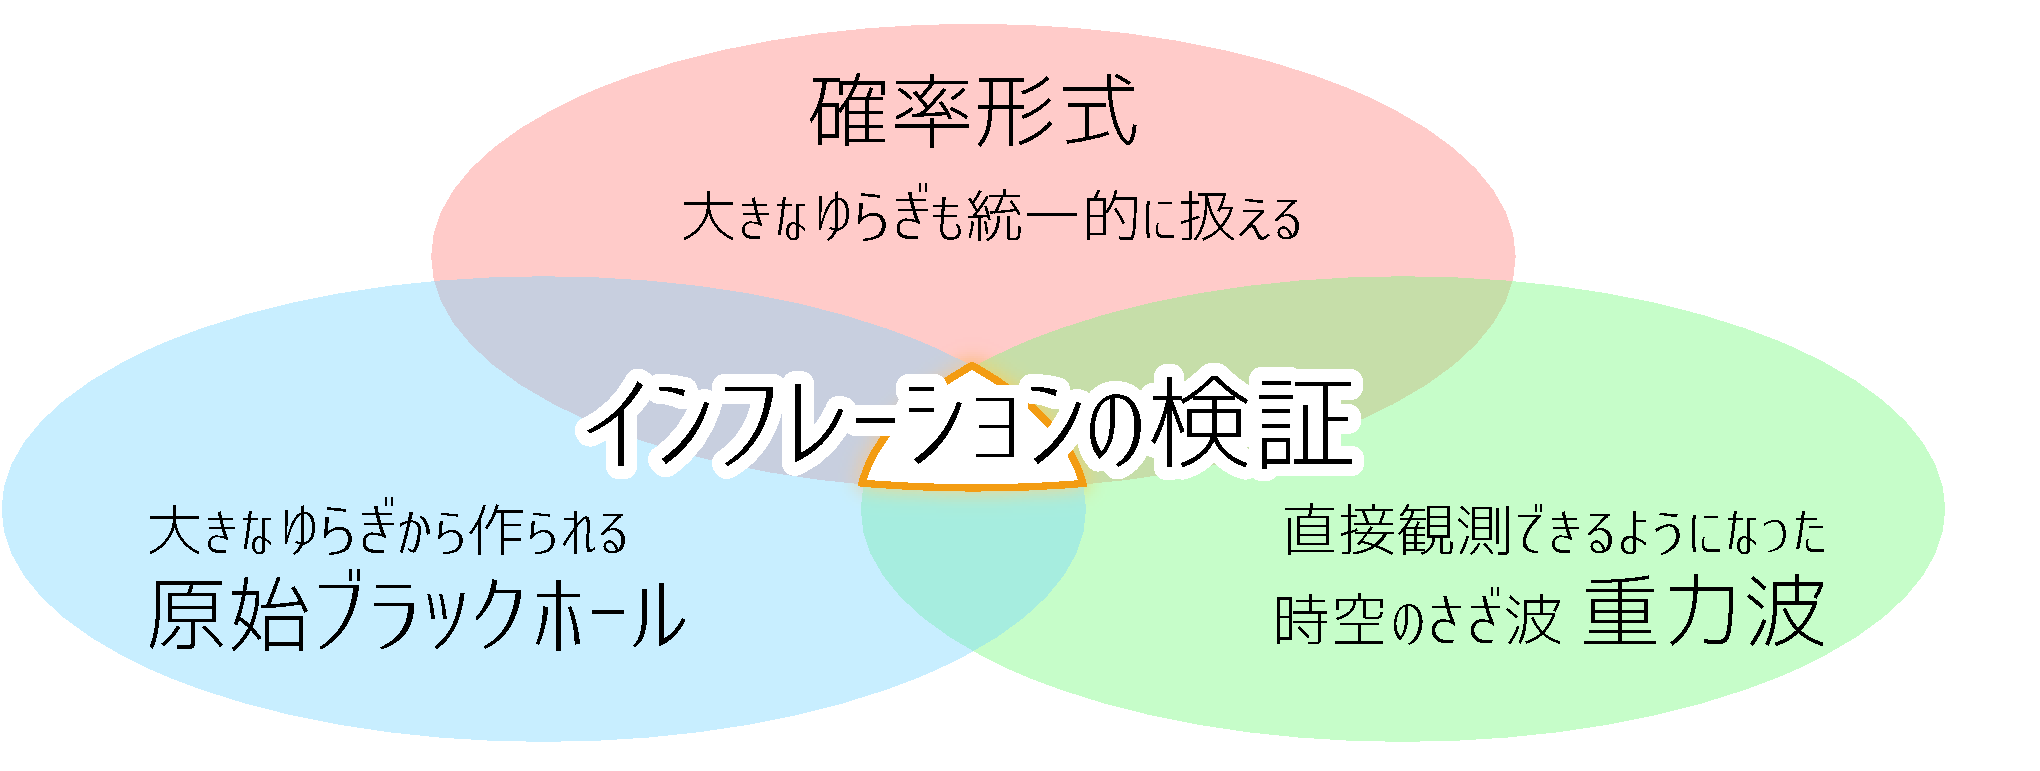
\includegraphics[width=0.7\hsize]{YLC2020_abstract.pdf}
	\caption{本研究の3つの要素と最終目的.}
	\label{fig: abstract}
\end{figure}



	
\vspace*{1zw}	% (概要)と(本文)の間が10行程度になるよう、必要に応じて値を調整してください。	
%end 研究目的及び研究計画の概要空行付き ====================

\noindent
\rule{\linewidth}{1pt}\\
\noindent
\textbf{(本文)}
%begin 研究目的と研究計画 ====================
%\JSPSInstructions	% <-- 留意事項。これは消すか、コメントアウトしてください。

\begin{mdframed}[roundcorner=0.5zw,
	%skipabove=1zw,skipbelow=1zw,
	innertopmargin=0.8zw,innerbottommargin=0.8zw,
	%innerleftmargin=0.8zw,innerrightmargin=0.8zw,
	%rightmargin=5000pt,leftmargin=50pt,
	linecolor=black!50,linewidth=0.2zw,
	backgroundcolor=black!10]
	{\bfseries\gtfamily\sffamily\large 1. 研究の学術的背景および核心となる「問い」}
\end{mdframed}

\noindent
現代宇宙論では, 宇宙最初期に\emph{インフレーション}と呼ばれる加速膨張が起こったことが広く支持されている.
インフレーションは大局的には宇宙を均一にしつつ, 量子力学的効果で細かな空間の歪み (曲率ゆらぎ) も作ることが知られており, 
その歪みに物質が集まることで現在の銀河等宇宙構造のもとになると考えられている.
インフレーションは最初期であるがゆえ, 最高エネルギーを実現しているともされ,
宇宙論的観点だけでなく素粒子理論などの高エネルギー物理の観点からも「\ul{インフレーションの具体的な仕組みは何か?}」ということは
重要な学術的問いである.
近年 Planck 衛星によって初期宇宙のなごりの光 (宇宙背景放射; CMB) が精密に測定され~\cite{Planck:2013jfk},
インフレーション機構はさらに強く支持されるようになったが, その具体的な仕組みは未だ解明されていない.
むしろ Planck 衛星の詳細な観測により有力視されていた簡潔な理論の多くは否定されてしまい, 
より複雑で現実的な理論も視野に入れる必要が出てきているのが現状である.

一方インフレーションにも関係する明るい話題として, これまで間接的な証拠しかなかった\emph{重力波 (時空のさざ波)} が, 
LIGO/Virgo グループによって初めて直接観測された~\cite{Abbott:2016blz}. 
続く LISA などの重力波観測の人工衛星計画も視野に入り, 「\ul{重力波を用いて何が探求できるか?}」を議論することが
現在喫緊の課題となっている.
観測された重力波はブラックホールや中性子星の合体から生じたものであるが, 
太陽の 30 倍を超える重いブラックホールも多く見つかっており, そのような「\ul{重いブラックホールの生成機構}」は明らかになっていない.
それを受け, 通常とは異なる生成機構を持つ\emph{原始ブラックホール}が再注目されている. 
ブラックホールは通常重い恒星の爆発によって形成されるが, インフレーションで大きな曲率ゆらぎが作られた場合, 
宇宙初期にエネルギー密度の濃い領域が直接潰れることでも形成され, これを原始ブラックホールと呼ぶ. 
原始ブラックホールはいまだに発見されていないが, もし観測されればインフレーション理論の大きな情報となる. 
さらに原始ブラックホールは重力波源となるだけでなく, いまだ「\ul{正体の明らかになっていない暗黒物質}」の候補でもあり, 天体そのものとしても興味深い.




\begin{mdframed}[roundcorner=0.5zw,
	%skipabove=1zw,skipbelow=1zw,
	innertopmargin=0.8zw,innerbottommargin=0.8zw,
	%innerleftmargin=0.8zw,innerrightmargin=0.8zw,
	%rightmargin=5000pt,leftmargin=50pt,
	linecolor=black!50,linewidth=0.2zw,
	backgroundcolor=black!10]
	{\bfseries\gtfamily\sffamily\large 2. 研究の目的および学術的独自性}
\end{mdframed}

\noindent
以上の背景を踏まえ本研究課題では, \emph{インフレーションの確率形式・原始ブラックホール・重力波}を三位一体とした
「\ul{インフレーション理論の包括的解析}」を主目的とし,
また派生として「\ul{暗黒物質や初期宇宙の物理を調査}」することを副目的とする.

インフレーションの確率形式は量子効果由来のインフレーションのゆらぎを古典的乱数で近似して扱う手法である.
通常の摂動論的量子計算ではインフレーションのゆらぎが小さい場合しか扱うことができないが,
確率形式にて古典乱数として近似してしまえば大きなゆらぎであっても統一的に扱うことができる.
したがって大きなゆらぎ由来の天体である原始ブラックホールの生成などについて議論する際に必要不可欠である.
原始ブラックホールは\ul{暗黒物質}の候補であるし, また合体から生じる重力波を通じて検証可能性もある.
さらにもし原始ブラックホールを作るほどインフレーションのゆらぎが大きかった場合,
原始ブラックホールの合体からだけでなく, 初期宇宙において曲率ゆらぎの振動からも\emph{重力波が誘導}されることが知られている~\cite{Saito:2008jc}.
そのような誘導重力波は生成時の\ul{初期宇宙プラズマの情報を記録}している可能性がある~(3-\cite{Abe:2020sqb}).

そこで本研究課題ではインフレーションの理論的側面として確率形式に着目, 本形式を整備し, 
ゆらぎが大きくなる理論まで含めインフレーション理論の統一的解析を行う.
また観測的側面として, 確率形式を応用し原始ブラックホールや関連重力波量の正確な計算を行い, インフレーション理論の検証に役立てる.
確率形式を応用することで\ul{これまで計算できなかった大きなゆらぎやその派生である原始ブラックホール・重力波の正確な計算が可能になる}こと,
および\ul{理論から観測的検証までを一まとめ}にしてインフレーション機構に迫ることが, 本研究の学術的独自性である.


\begin{mdframed}[roundcorner=0.5zw,
	%skipabove=1zw,skipbelow=1zw,
	innertopmargin=0.8zw,innerbottommargin=0.8zw,
	%innerleftmargin=0.8zw,innerrightmargin=0.8zw,
	%rightmargin=5000pt,leftmargin=50pt,
	linecolor=black!50,linewidth=0.2zw,
	backgroundcolor=black!10]
	{\bfseries\gtfamily\sffamily\large 3. 研究の具体的計画}
\end{mdframed}

\noindent
本研究の具体的計画について, 確率形式・原始ブラックホール・重力波の3題目に分けて, 以下に詳細に記す.

\stochastic{インフレーションの確率形式}
申請者はすでにインフレーションの確率形式を応用し, 実際に大きな曲率ゆらぎにも適用できる計算手法の確立に成功している~(3-\cite{Fujita:2013cna,Fujita:2014tja}).
しかしながら本手法の具体的計算には大量の確率標本を数値的に生成する必要があり, 他の研究者が簡単に実装できるものではなかった. 
2015年に共同研究者でもある \emph{Vincent Vennin 氏 (APC 研究員)} らが本手法を偏微分方程式に焼き直し~\cite{Vennin:2015hra}, 
いくつかの解析解を与えるとともに, 統一的な数値実装の可能性を示した. そこで我々は現在共同で, 本手法を誰でも簡単に利用できるよう, 
公開プログラムとしての数値実装を進めている. 
これにより計算機によるインフレーション理論の自動解析が可能になり, クラスター計算機と組み合わせれば大規模な包括的探査も可能となるだろう.
具体的研究計画としてまず「\ul{確率的計算プログラムの完成・公開}」が挙げられる

プログラムの完成後は実際に様々なインフレーション理論に適用し解析を行っていく. 詳細は割愛するが, 特に近年幾何学力によって不安定性が生じる理論 
(\cite{Renaux-Petel:2015mga}等) とスローロール条件を破る理論 (\cite{Ezquiaga:2018gbw}等) に対し, 
ゆらぎが大きくなり確率形式が必須となる可能性が指摘され注目されている.
2つ目の研究計画はこのような「\ul{具体的なインフレーション理論に対し確率計算プログラムを適用し解析を行う}」ことである.

最後に原始ブラックホール生成量計算への応用が挙げられる.
原始ブラックホール生成量はゆらぎの大きさだけでなくその統計性にも大きく依存することが指摘されており (\cite{Ezquiaga:2019ftu}等),
その正確な計算には「\ul{我々の確率計算手法を様々な統計量に適用できるように拡張}」する必要がある.
これが3つ目の研究計画である. 申請者はすでに, 曲率ゆらぎの高次統計量を計算する手法について準備研究を行なっており~\cite{Tada:2016pmk,Suyama:2020akr}, これを応用すればよい.

\medskip


\PBH{原始ブラックホール}
原始ブラックホールに関しては, まず上述した拡張確率形式を応用して「\ul{原始ブラックホール生成量の正確な計算法を確立}」する研究を行う.
またゆらぎの高次統計量由来の原始ブラックホールの空間分布にも着目したい.
申請者はこれまでに, ゆらぎが高次統計量を持つと原始ブラックホールが密集して形成されることを指摘したが~(3-\cite{Tada:2015noa}),
これはブラックホール合体の歴史に影響し, したがって合体重力波によって区別できる可能性がある.
そこで「\ul{ゆらぎの統計性 {$\leftrightarrow$} 形成時の原始ブラックホール空間分布 {$\leftrightarrow$} 現在の合体重力波スペクトルの対応を明確に定式化}」し, 
重力波から原始ブラックホールを通じてインフレーション理論の情報を得る手段とする.

\medskip


\GW{重力波}
原始ブラックホールが形成されるほど曲率ゆらぎが大きかったとすると, ブラックホールの合体からだけでなく, 曲率ゆらぎの振動からも初期宇宙において
重力波が誘導生成されることが知られている. したがってこの誘導重力波を観測することで原始ブラックホールの間接的証拠とすることができる.
さらに興味深いことに合体ブラックホールとしてちょうど良い太陽質量程度の原始ブラックホールの形成は, 
初期宇宙でちょうど量子色力学 (QCD) の相転移が起こっている時代である.
加えて対応する誘導重力波の波数はパルサータイミングアレイ (PTA) と呼ばれる重力波観測法で観測可能な波数にちょうど一致している.
先日 NANOGrav グループがこの PTA を用いた重力波観測に初めて成功した可能性があることを発表し注目されている~\cite{Arzoumanian:2020vkk}.
このような状況のもと申請者はこれまで所属研究室である名古屋大学宇宙論研究室の大学院生らとともに,
この誘導重力波が QCD プラズマ流体の音速の変化に影響されることを示す研究を行った~(3-\cite{Abe:2020sqb}).
本研究では引き続き大学院生らとともに, NANOGrav 等の「\ul{具体的観測を考慮して初期宇宙プラズマの性質の観測可能性を定量的に議論する}」ことを計画している.
本研究はインフレーション理論の観点からだけでなく, QCD 理論等の素粒子原子核理論の立場からも重要である.

\bigskip



\begin{thebibliography}{99}

\scriptsize % フォントサイズを下げる
\setlength{\itemsep}{-2pt} % 行間を縮める

%\cite{Planck:2013jfk}
\bibitem{Planck:2013jfk}
P.~A.~R.~Ade \textit{et al.} [Planck],
%``Planck 2013 results. XXII. Constraints on inflation,''
Astron. Astrophys. \textbf{571}, A22 (2014).
%doi:10.1051/0004-6361/201321569
%[arXiv:1303.5082 [astro-ph.CO]].
%1740 citations counted in INSPIRE as of 28 Oct 2020

%\cite{Abbott:2016blz}
\bibitem{Abbott:2016blz}
B.~P.~Abbott \textit{et al.} [LIGO Scientific and Virgo],
%``Observation of Gravitational Waves from a Binary Black Hole Merger,''
Phys. Rev. Lett. \textbf{116}, no.6, 061102 (2016).
%doi:10.1103/PhysRevLett.116.061102
%[arXiv:1602.03837 [gr-qc]].
%5701 citations counted in INSPIRE as of 28 Oct 2020

%\cite{Saito:2008jc}
\bibitem{Saito:2008jc}
R.~Saito and J.~Yokoyama,
%``Gravitational wave background as a probe of the primordial black hole abundance,''
Phys. Rev. Lett. \textbf{102}, 161101 (2009)
[erratum: Phys. Rev. Lett. \textbf{107}, 069901 (2011)].
%doi:10.1103/PhysRevLett.102.161101
%[arXiv:0812.4339 [astro-ph]].
%142 citations counted in INSPIRE as of 28 Oct 2020

%\cite{Vennin:2015hra}
\bibitem{Vennin:2015hra}
V.~Vennin and A.~A.~Starobinsky,
%``Correlation Functions in Stochastic Inflation,''
Eur. Phys. J. C \textbf{75}, 413 (2015).
%doi:10.1140/epjc/s10052-015-3643-y
%[arXiv:1506.04732 [hep-th]].
%87 citations counted in INSPIRE as of 28 Oct 2020

%\cite{Renaux-Petel:2015mga}
\bibitem{Renaux-Petel:2015mga}
S.~Renaux-Petel and K.~Turzy\'nski,
%``Geometrical Destabilization of Inflation,''
Phys. Rev. Lett. \textbf{117}, no.14, 141301 (2016).
%doi:10.1103/PhysRevLett.117.141301
%[arXiv:1510.01281 [astro-ph.CO]].
%67 citations counted in INSPIRE as of 28 Oct 2020

%\cite{Ezquiaga:2018gbw}
\bibitem{Ezquiaga:2018gbw}
J.~M.~Ezquiaga and J.~Garc\'\i{}a-Bellido,
%``Quantum diffusion beyond slow-roll: implications for primordial black-hole production,''
JCAP \textbf{08}, 018 (2018).
%doi:10.1088/1475-7516/2018/08/018
%[arXiv:1805.06731 [astro-ph.CO]].
%49 citations counted in INSPIRE as of 28 Oct 2020

%\cite{Ezquiaga:2019ftu}
\bibitem{Ezquiaga:2019ftu}
J.~M.~Ezquiaga, J.~Garc\'\i{}a-Bellido and V.~Vennin,
%``The exponential tail of inflationary fluctuations: consequences for primordial black holes,''
JCAP \textbf{03}, 029 (2020).
%doi:10.1088/1475-7516/2020/03/029
%[arXiv:1912.05399 [astro-ph.CO]].
%16 citations counted in INSPIRE as of 28 Oct 2020

%\cite{Tada:2016pmk}
\bibitem{Tada:2016pmk}
\me and V.~Vennin,
%``Squeezed bispectrum in the $\delta N$ formalism: local observer effect in field space,''
JCAP \textbf{02}, 021 (2017)
doi:10.1088/1475-7516/2017/02/021
[arXiv:1609.08876 [astro-ph.CO]].
%16 citations counted in INSPIRE as of 29 Oct 2020

%\cite{Suyama:2020akr}
\bibitem{Suyama:2020akr}
T.~Suyama, \me and M.~Yamaguchi,
%``Local observer effect on the cosmological soft theorem,''
[arXiv:2008.13364 [astro-ph.CO]].
%2 citations counted in INSPIRE as of 29 Oct 2020

%\cite{Arzoumanian:2020vkk}
\bibitem{Arzoumanian:2020vkk}
Z.~Arzoumanian \textit{et al.} [NANOGrav],
%``The NANOGrav 12.5-year Data Set: Search For An Isotropic Stochastic Gravitational-Wave Background,''
[arXiv:2009.04496 [astro-ph.HE]].
%36 citations counted in INSPIRE as of 28 Oct 2020

\end{thebibliography}



%end 研究目的と研究計画 ====================

% p01_purpose_plan_01.tex
\KLEndSubject{F}


%#Split: 02_background  
%#PieceName: p02_background
% p02_background_00.tex
\KLBeginSubject{02}{2}{2 本研究の着想に至った経緯など}{1}{F}{}{jsps-subject-header}{jsps-default-header}

\section{2 本研究の着想に至った経緯など}
%    <<最大 1ページ>>

%s03_background
%begin 本研究の着想に至った経緯など ====================
		
\begin{mdframed}[roundcorner=0.5zw,
	%skipabove=1zw,skipbelow=1zw,
	innertopmargin=0.8zw,innerbottommargin=0.8zw,
	%innerleftmargin=0.8zw,innerrightmargin=0.8zw,
	%rightmargin=5000pt,leftmargin=50pt,
	linecolor=black!50,linewidth=0.2zw,
	backgroundcolor=black!10]
	{\bfseries\gtfamily\sffamily\large 1. 着想に至った経緯と準備状況}
\end{mdframed}

\noindent
本来インフレーションの確率形式ではインフレーション場のゆらぎのみが計算され, 宇宙構造のもととなる曲率ゆらぎを直接計算することはできなかった.
これに対し, 曲率ゆらぎとインフレーション時間のゆらぎを対応づける $\delta N$ 形式を応用することで曲率ゆらぎを直接計算することができることを発見したこと,
また我々の計算手法を数学的に整備した Vennin 氏らの研究により数値計算の可能性が開けたことが, 本研究の着想に至った経緯である.
以降イギリスの \emph{David Wands 氏 (ICG 教授)} らにより原始ブラックホールへの応用や (\cite{Pattison:2017mbe} 等), 
オランダの \emph{Tomislav Prokopec 氏 (Utrecht 准教授)} らによりスローロール近似を超えた適用などが議論され (\cite{Prokopec:2019srf} 等),
特にヨーロッパを中心に注目を集めている.
一方原始ブラックホールやその間接的証拠としての誘導重力波はすでに世界的に注目されており,
また原始ブラックホール生成に対する QCD 相転移の影響も議論されていたが~\cite{Byrnes:2018clq},
誘導重力波に対する相転移の影響は見逃されていた.
大学院生の指導の一環として QCD 相転移と誘導重力波の関係について研究を始めたことがもう1つの経緯である.

準備状況としては, 確率計算プログラムに関してその大枠は完成しており, 
またフランスでのポスドク研究員時代からの確率形式の理論的整備に関する研究も先日完成したため~(3-\cite{Pinol:2018euk,Pinol:2020cdp}),
数値プログラムの準備は完了し, あとは性能確認と使用手引きを完成させるだけである.
原始ブラックホールにも応用されるゆらぎの統計量の拡張についても, 準備研究をいくつか発表し~(1-\cite{Tada:2016pmk,Suyama:2020akr}),
現在も共同研究者らとともに議論を進めている.
原始ブラックホール形成理論についても申請者は多くの研究を積んでいる~(3-\cite{Kawasaki:2016pql,Inomata:2016rbd,Inomata:2017okj,Inomata:2017uaw} 等).
大学院生らとの誘導重力波の研究に関しても先日最初の論文を発表することができた~(3-\cite{Abe:2020sqb}).
本研究の準備は順調に進んでいると言える.


\begin{mdframed}[roundcorner=0.5zw,
	%skipabove=1zw,skipbelow=1zw,
	innertopmargin=0.8zw,innerbottommargin=0.8zw,
	%innerleftmargin=0.8zw,innerrightmargin=0.8zw,
	%rightmargin=5000pt,leftmargin=50pt,
	linecolor=black!50,linewidth=0.2zw,
	backgroundcolor=black!10]
	{\bfseries\gtfamily\sffamily\large 2. 本研究の世界的位置付け}
\end{mdframed}

\noindent
申請者らの曲率ゆらぎ計算手法の提唱や, Vennin 氏らの数学的整備の研究を受け, 現在インフレーションの確率形式は特にヨーロッパを中心として注目を集めている.
原始ブラックホールは LIGO/Virgo による合体重力波検出から世界的に注目されており, 誘導重力波も NANOGrav の発表を受け関連研究が多く発表されている.
ところがそれぞれに特化した研究は多くなされているものの, これらを統合した研究はほとんど行われていない.
これは特に確率形式の理解が浸透しきっていないためである.
そこで確率形式手法の提唱者であり原始ブラックホールや重力波についても研究を重ねてきた申請者が, 
その統合研究を先導することは重要であると考えられる.
そしてインフレーションの理論から観測までを一まとめにした本研究を
\ul{インフレーション研究の新たな分野に押し進める}ことを目指す.
また誘導重力波を通して初期宇宙を素粒子原子核の「実験場」として利用する考え方は,
高エネルギー物理に新たな情報を与えることができるだけでなく,
日本および世界の重力波観測計画をさらに促進することができるであろう.




\bigskip

\begin{thebibliography}{99}

\scriptsize % フォントサイズを下げる
\setlength{\itemsep}{-2pt} % 行間を縮める

%\cite{Pattison:2017mbe}
\bibitem{Pattison:2017mbe}
C.~Pattison, V.~Vennin, H.~Assadullahi and D.~Wands,
%``Quantum diffusion during inflation and primordial black holes,''
JCAP \textbf{10}, 046 (2017).
%doi:10.1088/1475-7516/2017/10/046
%[arXiv:1707.00537 [hep-th]].
%66 citations counted in INSPIRE as of 29 Oct 2020

%\cite{Prokopec:2019srf}
\bibitem{Prokopec:2019srf}
T.~Prokopec and G.~Rigopoulos,
%``$\Delta\mathcal{N}$ and the stochastic conveyor belt of Ultra Slow-Roll,''
[arXiv:1910.08487 [gr-qc]].
%5 citations counted in INSPIRE as of 29 Oct 2020

%\cite{Byrnes:2018clq}
\bibitem{Byrnes:2018clq}
C.~T.~Byrnes, M.~Hindmarsh, S.~Young and M.~R.~S.~Hawkins,
%``Primordial black holes with an accurate QCD equation of state,''
JCAP \textbf{08}, 041 (2018).
%doi:10.1088/1475-7516/2018/08/041
%[arXiv:1801.06138 [astro-ph.CO]].
%68 citations counted in INSPIRE as of 28 Oct 2020

\end{thebibliography}

		
		
%end 本研究の着想に至った経緯など ====================

% p02_background_01.tex
\KLEndSubject{F}


%#Split: 03_abilities  
%#PieceName: p03_abilities
% p03_abilities_00.tex
\KLBeginSubject{03}{3}{3 応募者の研究遂行能力及び研究環境}{2}{F}{}{jsps-subject-header}{jsps-default-header}

\section{3 応募者の研究遂行能力及び研究環境}
%    <<最大 2ページ>>

% s14_abilities
%begin 応募者の研究遂行能力及び研究環境 ====================
%\PapersInstructions	% <-- 研究業績留意事項。これは消すか、コメントアウトしてください。

\begin{mdframed}[roundcorner=0.5zw,
	%skipabove=1zw,skipbelow=1zw,
	innertopmargin=0.8zw,innerbottommargin=0.8zw,
	%innerleftmargin=0.8zw,innerrightmargin=0.8zw,
	%rightmargin=5000pt,leftmargin=50pt,
	linecolor=black!50,linewidth=0.2zw,
	backgroundcolor=black!10]
	{\bfseries\gtfamily\sffamily\large 1. これまでの研究活動}
\end{mdframed}

\noindent
申請者はこれまで\ul{21本の論文}を発表し, \ul{24件の国際会議}, \ul{22件の国内外研究所でのセミナー発表}を行なっている.
2019年にはブラジルとの2国間研究会 ``FAPESP-JSPS Workshop on dark energy, dark matter, and galaxies"
にて\ul{若手代表発表者として選出}され, 原始ブラックホールに関する発表を行った.
フェローシップとして\ul{フォトンサイエンス・リーディング大学院}や\ul{日本学術振興会特別研究員 DC2 および PD} に採用され,
\ul{科学研究費助成事業若手研究 (1回目)} にも採択されている.
これら研究資金を利用して海外経験も積み, 学生の時から海外研究者とも共同研究を行ってきた. 
2017 年度は\ul{フランス国立科学研究センター (CNRS) に PD 研究員として採用}されパリ天体物理学研究所 (IAP) に滞在していたが, 
特別研究員 PD に採用されたため任期途中で切り上げ帰国することとなり, 現在は名古屋大学に所属している.
今年度採用分の\ul{名古屋大学高等研究院 YLC 特任助教として内定}され, 来年度からも引き続き名古屋大学宇宙論研究室に所属し,
安定した研究活動と大学院生の研究指導を行うことができる.
その他の詳細な経歴については申請者の web ページ \url{https://nekomammat.github.io/indexJP.html}も参照されたい.

研究テーマは主にインフレーションに関連した初期宇宙の物理についてである.
最初の論文~\cite{Fujita:2013cna} ではインフレーションの確率形式において曲率ゆらぎを直接計算する手法を提唱し,
続く論文~\cite{Fujita:2014tja} では本手法を実際に, ゆらぎが大きくなって従来手法が破綻する理論に適用し, 初めて曲率ゆらぎの定量的な計算に成功した.
論文~\cite{Kawasaki:2015ppx} では当理論における原始ブラックホール形成も議論し, 現実的な確率形式の利用法を確立してきたと言える.
フランスポスドク時代には, これまで多くの研究者が利用してきた素朴なインフレーション確率形式の定式化では, 数学的に不定性があり,
より一般的なインフレーション理論に対して運動方程式が1つに定まらない問題があることを発見した~\cite{Pinol:2018euk}.
日本に戻ってきてからもフランスの共同研究者らと研究を続け, 先日ついに数学的に一意で, 一般的なインフレーション理論に対しても適用可能な
確率形式の定式化に成功し~\cite{Pinol:2020cdp}, インフレーション理論の大規模包括的解析の準備が整ったと言える.

原始ブラックホールについては一連の研究~\cite{Kawasaki:2016pql,Inomata:2016rbd,Inomata:2017okj,Inomata:2017uaw} が業界から注目されている.
原始ブラックホールの実現には大きな曲率ゆらぎが必要になる一方, 大規模スケール ($\gtrsim1\,\mathrm{Mpc}$) においては曲率ゆらぎが非常に小さかったことが CMB 等の宇宙観測からわかっており,
したがってこれまで原始ブラックホールを実現するインフレーション理論にはパラメータの細かい調整を必要とする不自然なものが多かった.
一方我々はインフレーションが2回以上起き, 大規模スケールと原始ブラックホールスケールのゆらぎが異なるインフレーションに対応していたとすれば, 非常に簡単に原始ブラックホールを実現できることを指摘した.
このような多段階インフレーションは, 量子重力理論の候補である超弦理論の文脈から支持されることも議論している~\cite{Kogai:2020jkq}.
同じく名古屋大学宇宙論研究室所属の\emph{横山修一郎氏 (名古屋大学助教)} とはこのような多段階インフレーションにて, LIGO/Virgo の合体ブラックホール, 暗黒物質, そして OGLE グループが発見した銀河中心に向けての正体不明の重力レンズ現象~\cite{Niikura:2019kqi}
の全てを原始ブラックホールで同時に説明することができること示した~\cite{Tada:2019amh}.
横山氏とはゆらぎの統計性が原始ブラックホールの密集形成に影響することも指摘し~\cite{Tada:2015noa}, これは合体重力波の頻度の観点からも重要である.

これまで申請者は現研究室で大学院生の研究指導にも積極的に貢献してきたが~\cite{Kogai:2020jkq,Mikura:2020qhc,Abe:2020sqb},
論文~\cite{Abe:2020sqb} では大学院生らとともに, 誘導重力波が QCD 相転移プラズマの音速の変化に影響されることを示し, 
したがって誘導重力波の詳細な観測によって初期宇宙の QCD 相転移プラズマの性質を探り得る可能性があることを示唆した.
引き続き具体的な重力波観測計画を考慮し, プラズマパラメータの観測可能性を定量的に議論する研究を行う予定である.

以上が申請者のこれまでの研究活動と実績の簡単なまとめであり, 本研究課題の遂行可能性を示す客観的証拠であると言える.


\begin{mdframed}[roundcorner=0.5zw,
	%skipabove=1zw,skipbelow=1zw,
	innertopmargin=0.8zw,innerbottommargin=0.8zw,
	%innerleftmargin=0.8zw,innerrightmargin=0.8zw,
	%rightmargin=5000pt,leftmargin=50pt,
	linecolor=black!50,linewidth=0.2zw,
	backgroundcolor=black!10]
	{\bfseries\gtfamily\sffamily\large 2. 研究環境}
\end{mdframed}

\noindent
名古屋大学高等研究院の YLC 特任助教に内定されたため, 引き続き名古屋大学宇宙論研究室で安定した研究活動が可能である.
当研究室においてすでに研究者および大学院生らとの共同研究実績を挙げており, 本研究課題に対して研究環境が適していることを示している.
特に原始ブラックホールに関しては当分野を先導している横山氏や\emph{柳哲文氏 (名古屋大学講師)} の助けを借りることができるため, 非常に優れた研究環境だと言える.
確率形式の大規模計算に対して, 当研究室はクラスター計算機 ``galaxy" を所有しており研究に役立つであろう.
また本研究課題は国内においては\emph{藤田智弘氏 (東京大学研究員)} や\emph{徳田順生氏 (神戸大学研究員)} との共同研究を計画しており,
名古屋大学は各研究所に対し地理的に中心に位置しているため, 共同研究を進めやすい.
国外研究者としてはフランスの共同研究者である Vennin 氏や \emph{S\'ebastien Renaux-Petel 氏 (IAP 研究員)}, \emph{Lucas Pinol 氏 (IAP 大学院生)} との引き続きの共同研究はもちろん,
イギリスの Wands 氏や \emph{Christian Byrnes 氏 (Sussex 上級主任研究員)}, イタリアの \emph{Sabino Matarrese 氏 (Padova 教授)} や \emph{Nicola Bartolo 氏 (Padova 准教授)}
との議論および協力を予定している (実際直近では 2020 年 11 月に Padova グループでのオンラインセミナー発表を依頼されている).
普段は電子メールやオンライン会議, チャットツールを駆使して連絡をとっているが, より円滑な共同研究活動のためには旅費や設備準備費として本科学研究費が必要不可欠である.



\bigskip

\begin{thebibliography}{99}

\scriptsize % フォントサイズを下げる
\setlength{\itemsep}{-2pt} % 行間を縮める

%\cite{Fujita:2013cna}
\bibitem{Fujita:2013cna}
T.~Fujita, M.~Kawasaki, \me and T.~Takesako,
%``A new algorithm for calculating the curvature perturbations in stochastic inflation,''
JCAP \textbf{12}, 036 (2013).
%doi:10.1088/1475-7516/2013/12/036
%[arXiv:1308.4754 [astro-ph.CO]].
%33 citations counted in INSPIRE as of 29 Oct 2020

%\cite{Fujita:2014tja}
\bibitem{Fujita:2014tja}
T.~Fujita, M.~Kawasaki and \me,
%``Non-perturbative approach for curvature perturbations in stochastic $\delta N$ formalism,''
JCAP \textbf{10}, 030 (2014).
%doi:10.1088/1475-7516/2014/10/030
%[arXiv:1405.2187 [astro-ph.CO]].
%33 citations counted in INSPIRE as of 29 Oct 2020

%\cite{Kawasaki:2015ppx}
\bibitem{Kawasaki:2015ppx}
M.~Kawasaki and \me,
%``Can massive primordial black holes be produced in mild waterfall hybrid inflation?,''
JCAP \textbf{08}, 041 (2016).
%doi:10.1088/1475-7516/2016/08/041
%[arXiv:1512.03515 [astro-ph.CO]].
%32 citations counted in INSPIRE as of 29 Oct 2020

%\cite{Pinol:2018euk}
\bibitem{Pinol:2018euk}
L.~Pinol, S.~Renaux-Petel and \me,
%``Inflationary stochastic anomalies,''
Class. Quant. Grav. \textbf{36}, no.7, 07LT01 (2019).
%doi:10.1088/1361-6382/ab097f
%[arXiv:1806.10126 [gr-qc]].
%17 citations counted in INSPIRE as of 29 Oct 2020

%\cite{Pinol:2020cdp}
\bibitem{Pinol:2020cdp}
L.~Pinol, S.~Renaux-Petel and \me,
%``A manifestly covariant theory of multifield stochastic inflation in phase space,''
[arXiv:2008.07497 [astro-ph.CO]].
%5 citations counted in INSPIRE as of 29 Oct 2020


%\cite{Kawasaki:2016pql}
\bibitem{Kawasaki:2016pql}
M.~Kawasaki, A.~Kusenko, \me and T.~T.~Yanagida,
%``Primordial black holes as dark matter in supergravity inflation models,''
Phys. Rev. D \textbf{94}, no.8, 083523 (2016).
%doi:10.1103/PhysRevD.94.083523
%[arXiv:1606.07631 [astro-ph.CO]].
%81 citations counted in INSPIRE as of 29 Oct 2020

%\cite{Inomata:2016rbd}
\bibitem{Inomata:2016rbd}
K.~Inomata, M.~Kawasaki, K.~Mukaida, \me and T.~T.~Yanagida,
%``Inflationary primordial black holes for the LIGO gravitational wave events and pulsar timing array experiments,''
Phys. Rev. D \textbf{95}, no.12, 123510 (2017).
%doi:10.1103/PhysRevD.95.123510
%[arXiv:1611.06130 [astro-ph.CO]].
%103 citations counted in INSPIRE as of 29 Oct 2020

%\cite{Inomata:2017okj}
\bibitem{Inomata:2017okj}
K.~Inomata, M.~Kawasaki, K.~Mukaida, \me and T.~T.~Yanagida,
%``Inflationary Primordial Black Holes as All Dark Matter,''
Phys. Rev. D \textbf{96}, no.4, 043504 (2017).
%doi:10.1103/PhysRevD.96.043504
%[arXiv:1701.02544 [astro-ph.CO]].
%92 citations counted in INSPIRE as of 29 Oct 2020

%\cite{Inomata:2017uaw}
\bibitem{Inomata:2017uaw}
K.~Inomata, M.~Kawasaki, K.~Mukaida, \me and T.~T.~Yanagida,
%``$\mathcal O(10) M_\odot$ primordial black holes and string axion dark matter,''
Phys. Rev. D \textbf{96}, no.12, 123527 (2017).
%doi:10.1103/PhysRevD.96.123527
%[arXiv:1709.07865 [astro-ph.CO]].
%7 citations counted in INSPIRE as of 29 Oct 2020

%\cite{Kogai:2020jkq}
\bibitem{Kogai:2020jkq}
K.~Kogai and \me,
%``Escape from the swampland with a spectator field,''
Phys. Rev. D \textbf{101}, no.10, 103514 (2020)
doi:10.1103/PhysRevD.101.103514
[arXiv:2003.06753 [astro-ph.CO]].
%0 citations counted in INSPIRE as of 29 Oct 2020

%\cite{Niikura:2019kqi}
\bibitem{Niikura:2019kqi}
H.~Niikura, M.~Takada, S.~Yokoyama, T.~Sumi and S.~Masaki,
%``Constraints on Earth-mass primordial black holes from OGLE 5-year microlensing events,''
Phys. Rev. D \textbf{99}, no.8, 083503 (2019).
%doi:10.1103/PhysRevD.99.083503
%[arXiv:1901.07120 [astro-ph.CO]].
%64 citations counted in INSPIRE as of 29 Oct 2020

%\cite{Tada:2019amh}
\bibitem{Tada:2019amh}
\me and S.~Yokoyama,
%``Primordial black hole tower: Dark matter, earth-mass, and LIGO black holes,''
Phys. Rev. D \textbf{100}, no.2, 023537 (2019).
%doi:10.1103/PhysRevD.100.023537
%[arXiv:1904.10298 [astro-ph.CO]].
%19 citations counted in INSPIRE as of 29 Oct 2020

%\cite{Tada:2015noa}
\bibitem{Tada:2015noa}
\me and S.~Yokoyama,
%``Primordial black holes as biased tracers,''
Phys. Rev. D \textbf{91}, no.12, 123534 (2015).
%doi:10.1103/PhysRevD.91.123534
%[arXiv:1502.01124 [astro-ph.CO]].
%48 citations counted in INSPIRE as of 29 Oct 2020


%\cite{Mikura:2020qhc}
\bibitem{Mikura:2020qhc}
Y.~Mikura, \me and S.~Yokoyama,
%``Conformal inflation in the metric-affine geometry,''
[arXiv:2008.00628 [hep-th]].
%1 citations counted in INSPIRE as of 29 Oct 2020

%\cite{Abe:2020sqb}
\bibitem{Abe:2020sqb}
K.~T.~Abe, \me and I.~Ueda,
%``Induced gravitational waves as a cosmological probe of the sound speed during the QCD phase transition,''
[arXiv:2010.06193 [astro-ph.CO]].
%0 citations counted in INSPIRE as of 29 Oct 2020

\end{thebibliography}


%end 応募者の研究遂行能力及び研究環境 ====================
%begin 研究業績リスト ====================
	%\begin{enumerate}
		%\paper{Search for whale eggs}{\yukawa\ \etal}{Rev.\ Oceanic Mysteries}{888}{99}{2017}
			%\label{pub:whale}
				
		%\paper{Theory of Elephant Eggs}{\yukawa, Kara Juzo \etal}{\prl}{800}{800-804}{2005}
			%\label{pub:theoegg}
				
		%\paper{仔象は死んだ}{Kobo Abe}{安部公房全集}{26}{100-200}{2004}
		
		%\paper{The Elephant's Child (象の鼻はなぜ長い)}{R.~Kipling}{Nature}{999}{777-799}{2003}

		%\paper{You can't Lay an Egg If You're an Elephant}{F.~Ehrlich}
			%{JofUR\\({\tt www.universalrejection.org})}{{\bf N/A}}{2002}
		
		% 下のように書いてもいいけど、めんどくさいし、表示の仕方を変えようとしたら大変。
		%\item ``Egg of Elephant-Bird'', 
				%\underline{A.~Cooper},
				%Nature, {\bf 409}, 704-707 (2001).	% 	
		%	\item Jack Torrance, ``All work and no play makes Jack a dull boy", The Shining (1980).
	\item \hspace{5mm}Jack Torrance, '`All work and no play makes Jack a dull boy", The Shining (1980).
	\item \hspace{10mm}Jack Torrance, ``All work and no play makes Jack a dull boy", The Shining (1980).
	\item \hspace{15mm}Jack Torrance, ``All work and no play makes Jack a dull boy", The Shining (1980).
	\item \hspace{20mm}Jack Torrance, ``All work and no play makes Jack a dull boy", The Shining (1980).
	\item \hspace{25mm}Jack Torrance, ``All work and no play makes Jack a dull boy", The Shining (1980).
	\item \hspace{30mm}Jack Torrance, ``All work and no play makes Jack a dull boy", The Shining (1980).
	\item \hspace{25mm}Jack Torrance, ``All work and no play makes Jack a dull boy", The Shining (1980).
	\item \hspace{20mm}Jack Torrance, ``All work and no play makes Jack a dull boy", The Shining (1980).
	\item \hspace{15mm}Jack Torrance, ``All work and no play makes Jack a dull boy", The Shining (1980).
	\item \hspace{10mm}Jack Torrance, ``All work and no play makes Jack a dull boy", The Shining (1980).
	\item \hspace{5mm}Jack Torrance, ``All work and no play makes Jack a dull boy", The Shining (1980).
	\item Jack Torrance, ``All work and no play makes Jack a dull boy", The Shining (1980).
	\item \hspace{5mm}Jack Torrance, ``All work and no play makes Jack a dull boy", The Shining (1980).
	\item \hspace{10mm}Jack Torrance, ``All work and no play makes Jack a dull boy", The Shining (1980).
	\item \hspace{15mm}Jack Torrance, ``All work and no play makes Jack a dull boy", The Shining (1980).
	\item \hspace{20mm}Jack Torrance, ``All work and no play makes Jack a dull boy", The Shining (1980).
	\item \hspace{25mm}Jack Torrance, ``All work and no play makes Jack a dull boy", The Shining (1980).
	\item \hspace{30mm}Jack Torrance, ``All work and no play makes Jack a dull boy", The Shining (1980).
	\item \hspace{25mm}Jack Torrance, ``All work and no play makes Jack a dull boy", The Shining (1980).
	\item \hspace{20mm}Jack Torrance, ``All work and no play makes Jack a dull boy", The Shining (1980).
	\item \hspace{15mm}Jack Torrance, ``All work and no play makes Jack a dull boy", The Shining (1980).
	\item \hspace{10mm}Jack Torrance, ``All work and no play makes Jack a dull boy", The Shining (1980).
	\item \hspace{5mm}Jack Torrance, ``All work and no play makes Jack a dull boy", The Shining (1980).
	\item Jack Torrance, ``All work and no play makes Jack a dull boy", The Shining (1980).
	\item \hspace{5mm}Jack Torrance, ``All work and no play makes Jack a dull boy", The Shining (1980).
	\item \hspace{10mm}Jack Torrance, ``All work and no play makes Jack a dull boy", The Shining (1980).
	\item \hspace{15mm}Jack Torrance, ``All work and no play makes Jack a dull boy", The Shining (1980).
	\item \hspace{20mm}Jack Torrance, ``All work and no play makes Jack a dull boy", The Shining (1980).
	% << only for demonstration. Please delete it or comment it out.
	%\end{enumerate}
%end 研究業績リスト ====================

% p03_abilities_01.tex
\KLEndSubject{F}


%#Split: 05_rights  
%#PieceName: p05_rights
% p05_rights_00.tex
\KLBeginSubject{04}{4}{4 人権の保護及び法令等の遵守への対応}{1}{F}{}{jsps-subject-header}{jsps-default-header}

\section{4 人権の保護及び法令等の遵守への対応}
%    <<最大 1ページ>>

% s09_rights
%begin 人権の保護及び法令等の遵守への対応 ====================
	
	\noindent
	該当しない.
	
%end 人権の保護及び法令等の遵守への対応 ====================

% p05_rights_01.tex
\KLEndSubject{F}


%#Split: 99_tail
% hook9 : right before \end{document} ============
 % pieces
\end{document}

